\section{Tactile switch}
\begin{figure}[H]
    \centering
    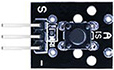
\includegraphics[angle=0, keepaspectratio=true, scale=1, width=200px, height=200px]{images/tactile.jpg}
    %\caption{Caption}
\end{figure}
\subsection*{Description}
This module is a simple tactile switch.
\subsection*{Pin mapping}
A tacticle switch is just a regular button switch.% Pressing the switch will short two sides of the switch and complete the circuit.
\begin{table}[H]
    \centering
    \begin{tabular}{|c|c|c|c|c|}
    \hline
    Index &Label &Type &Name &Description\\ \hline
    0 &S &Digital output &D0 &\\ \hline
    1 & &Source voltage &$V+$ &Unused\\ \hline
    2 &- &Ground &GND &\\ \hline
    \end{tabular}
    %\caption{Caption}
    %\label{tab:my_label}
\end{table}
\subsection*{Operation}
The digital output pin (D0) will be high when the switch is not pressed (open). When the button is pressed and the switch is closed D0 will be set to low.
%\subsection*{Code}
%\lstinputlisting[caption=test]{laser.py}